% =================================================

\begin{frame}
  \frametitle{Operating Receivers}


\begin{figure}
\begin{columns}
\column{.5\linewidth}
\begin{center}
  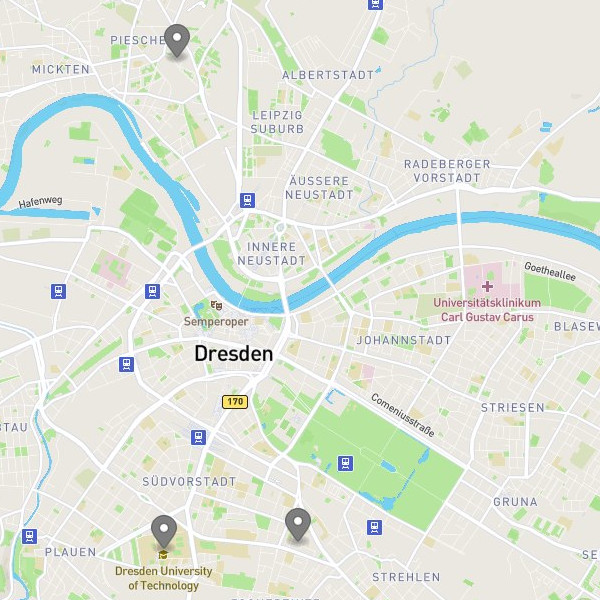
\includegraphics[height=0.65\textheight]{figs/map_dresden.jpg}
  \caption{Receivers in Dresden}
\end{center}
\column{.5\linewidth}
\begin{center}
  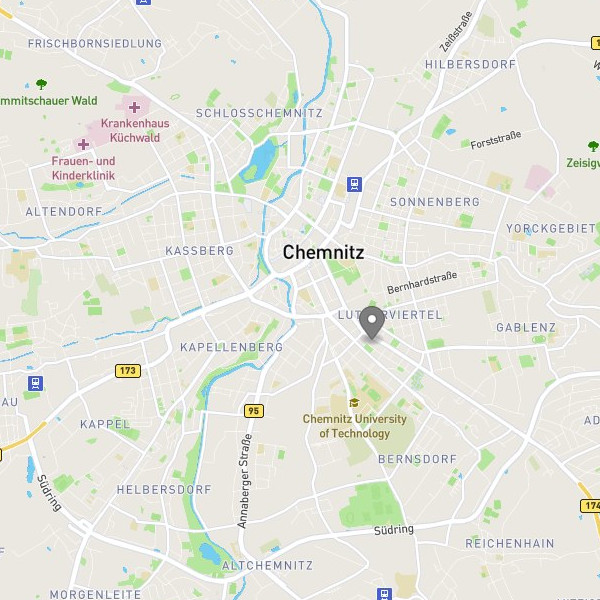
\includegraphics[height=0.65\textheight]{figs/map_chemnitz.jpg}
  \caption{Receivers in Chemnitz}
\end{center}
\end{columns}
\end{figure}

\end{frame}

% =================================================

\begin{frame}
\frametitle{Received Data}

\begin{figure}[h!]
  \begin{center}
    \begin{tikzpicture}[scale=0.6]
      \begin{axis}[
          width=\linewidth,
          grid=major,
          grid style={dashed,gray!30},
          xlabel=Time over 4 days,
          ylabel=Telegrams in 5 minute intervals,
          %x unit=time,
          %y unit=\si{\ampere},
          %legend style={at={(0.5,-0.2)},anchor=north},
          x tick label style={rotate=90,anchor=east},
          xticklabels={,,},
          %xticklabels={day1, day2, day3, day4} TODO: make nice labels
        ]
        \addplot
        table[x=time,y=value,col sep=comma] {figs/rawdata.csv};
      \end{axis}
    \end{tikzpicture}
  \end{center}
\end{figure}


\end{frame}

% =================================================

\begin{frame}
\frametitle{Assembeling a Receiver}

\begin{figure}
\begin{columns}
\column{.5\linewidth}
\begin{center}
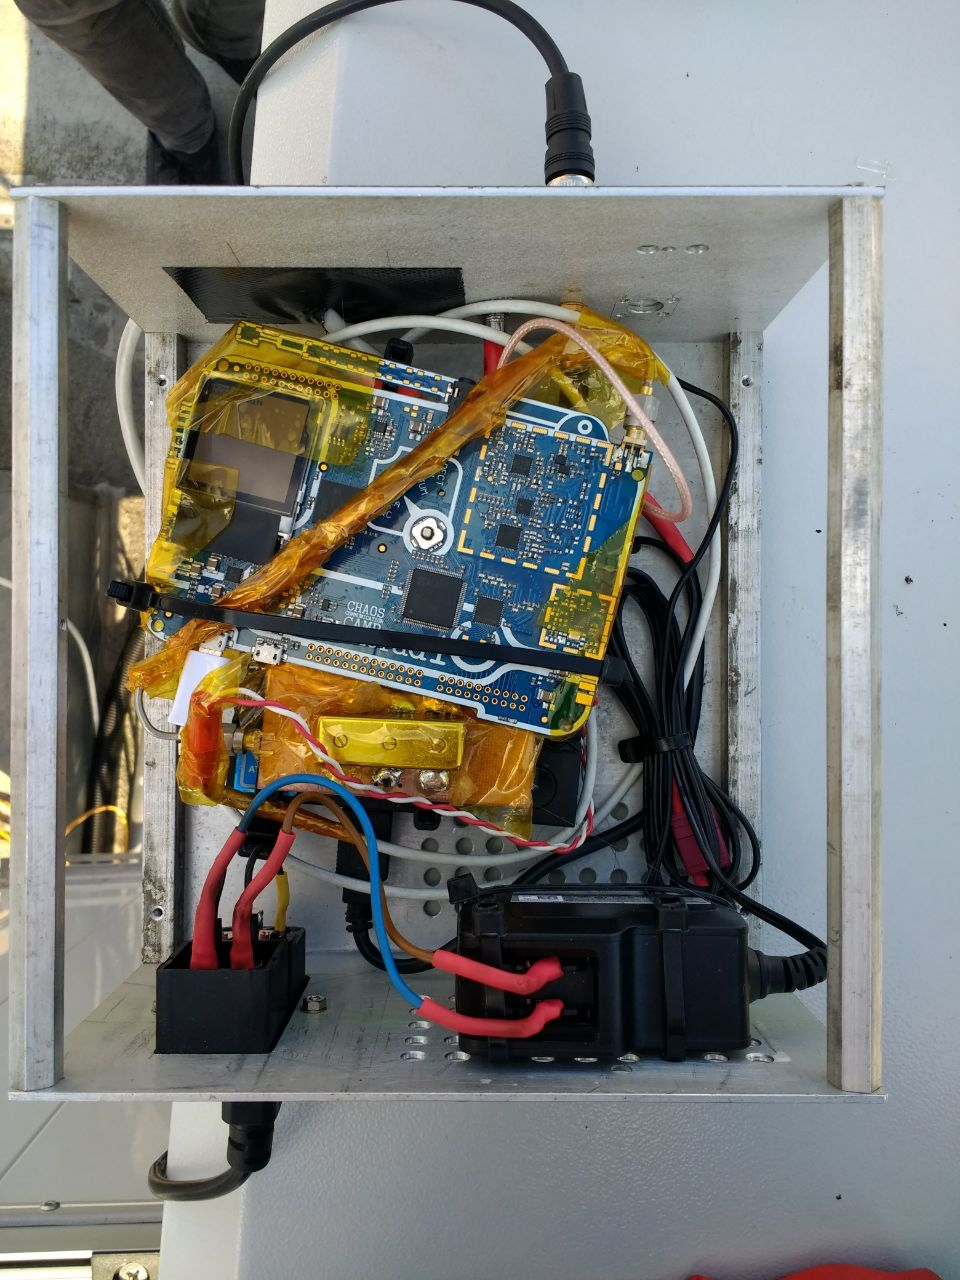
\includegraphics[height=0.7\textheight]{figs/station_barkhausen.jpg}
\end{center}
\column{.5\linewidth}
\raggedright
\caption{Station Barkhausenbau}
\vspace{0.5cm}

\begin{itemize}
	%\item\todo[inline]{make caption allign left}
	%\item\todo[inline]{please provide some details about this station}
  \item GDR powersuply casing (10\euro)
  \item Dell Wyse 3040 (70\euro)
  \item Rad1o Badge (e.g RTL SDR 30\euro)
  \item Hardware Filter (15\euro)
  \item Healthy amounts of kapton
\end{itemize}

$\Rightarrow$ ~130\euro \ per Station

\end{columns}
\end{figure}

\end{frame}

% =================================================

\begin{frame}
\frametitle{Architecture}

% Funnel
% DVB-API
% Clicky-Bunty
% Tracy

\usetikzlibrary{calc}
\usetikzlibrary{decorations.pathreplacing,decorations.markings,shapes.geometric}
\tikzset{radiation/.style={{decorate,decoration={expanding waves,angle=90,segment length=4pt}}}}

\begin{tikzpicture}[thick,scale=0.55, every node/.style={scale=0.55}]

% Station Box
\filldraw[draw=black,fill=lightgray] (0,3) rectangle (3,-3);

% GNU Radio and Telegram Decoder
\filldraw[draw=black,fill=gray] (0.1,0.8) rectangle (2.9,2.8);
\filldraw[draw=black,fill=gray] (0.1,-0.8) rectangle (2.9,-2.8);

% Data Flow
\draw[->,rounded corners, line width=0.25mm, red] (1.5, 0.8) -- (1.5,-0.8);

% Antenna Drawing
\draw[rounded corners, line width=0.25mm, black] (3, 1.8) -- (4,1.8) -- (4, 4);
\draw[radiation,decoration={angle=45}] (4,4) -- +(180:1);
\draw[radiation,decoration={angle=45}] (4,4) -- +(0:1);

% Labeling
\node[text width=2cm] at (1.5,1.8) {GNU-Radio};
\node[text width=2cm] at (1.5,-1.8) {\centering Telegram Decoder};

\node[text width=0.2cm] at (1.7,0) {\tiny UDP};

\filldraw[draw=black,fill=white] (5,3) rectangle (19,-3);

\filldraw[draw=black,fill=lightgray] (5.5,1) rectangle (9,-1);
\node[database,label=above:postgres,database radius=0.7cm,database segment height=0.35cm] at (10,-2) {};
\node[database,label=above:stops.json,database radius=0.7cm,database segment height=0.35cm] at (10,0.5) {};

% DataAccm <-> Postgres
\draw[<->,rounded corners, line width=0.25mm] (6, -1)  -- (6,-2) -- (9.2,-2);
%\draw[->,rounded corners, line width=0.25mm] (9.2, -1.9)  -- (6.1,-1.9) -- (6.1,-1);

% User Facing Services
\filldraw[draw=black,fill=lightgray] (15,2.9) rectangle (18.5,1.6);
\filldraw[draw=black,fill=lightgray] (15,1.4) rectangle (18.5,0.1);
\filldraw[draw=black,fill=lightgray] (15,-0.1) rectangle (18.5,-1.4);
\filldraw[draw=black,fill=lightgray] (15,-1.6) rectangle (18.5,-2.9);

% GRPC Arrows
% 1f77b4 31 119 180
\draw[->,rounded corners, draw={rgb:red,31;green,119;blue,180}, line width=0.25mm] (6, 1)  -- (6,2.25) -- (15,2.25);
\draw[->,rounded corners, draw={rgb:red,31;green,119;blue,180}, line width=0.25mm] (12.7, 2.25)  -- (12.7,0.9) -- (15,0.9);

% Postgres Arrows
% Tracy
\draw[<->,rounded corners, line width=0.25mm] (10.8, -2.2)  -- (15,-2.2);
%\draw[->,rounded corners, line width=0.25mm] (15, -2.3)  -- (10.8,-2.3);
% Clicky-Bunty-Server
\draw[<->,rounded corners, line width=0.25mm] (15, -0.8)  -- (12.9, -0.8) -- (12.9, -2.1) -- (10.8,-2.1);
%\draw[->,rounded corners, line width=0.25mm] (10.8, -2)  -- (12.8, -2) -- (12.8, -0.7) -- (15,-0.7);
% DVB-API
\draw[->,rounded corners, line width=0.25mm] (10.8, -1.9)  -- (12.7, -1.9) -- (12.7, 0.6) -- (15, 0.6);

% Labeling
\node[text width=3cm] at (7.3,0) {Data-Accumulator};
\node[text width=2cm] at (16.75,2.25) {Funnel};
\node[text width=2cm] at (16.8,0.75) {DVB-API};
\node[text width=2.5cm] at (16.8,-0.75) {Clicky-Bunty};
\node[text width=1cm] at (16.75,-2.25) {Tracy};

% Look Ups
\draw[->,rounded corners, draw={rgb:red,255;green,127;blue,14}, line width=0.25mm] (10.8, 0.75)  -- (15, 0.75);

% Labeling Arrows
\node[text width=2cm] at (11.7,2.5) {\tiny GRPC/Protobuf};
\node[text width=1cm] at (11.7,1) {\tiny Look UP};
\node[text width=1cm] at (11.7, -1.7) {\tiny Queries};

% ff7f0e 255 127 14
\draw[->,rounded corners, draw={rgb:red,255;green,127;blue,14}, line width=0.25mm] (4.75, 0)  -- (5.5, 0);


% Station Box
\filldraw[draw=black,fill=white] (21,3) rectangle (24,-3);

% GNU Radio and Telegram Decoder
\filldraw[draw=black,fill=lightgray] (21.1,0.1) rectangle (23.9,2.9);
\filldraw[draw=black,fill=lightgray] (21.1,-0.1) rectangle (23.9,-1.4);
\filldraw[draw=black,fill=lightgray] (21.1,-1.6) rectangle (23.9,-2.9);

% Labeling
\node[text width=2cm] at (23,1.5) {Map};
\node[text width=2cm] at (23,-0.75) {Click};
\node[text width=2cm] at (23,-2.25) {Tracy};

\draw[->,rounded corners, draw={rgb:red,255;green,127;blue,14}, line width=0.25mm] (18.5, 2.25)  -- (21, 2.25);

\draw[->,rounded corners, draw={rgb:red,255;green,127;blue,14}, line width=0.25mm] (18.5, 0.75)  -- (21, 0.75);

\draw[<->,rounded corners, draw={rgb:red,255;green,127;blue,14}, line width=0.25mm] (21, -0.7)  -- (18.5, -0.7);
%\draw[->,rounded corners, draw={rgb:red,255;green,127;blue,14}, line width=0.25mm] (18.5, -0.8)  -- (21, -0.8);

\draw[<->,rounded corners, draw={rgb:red,255;green,127;blue,14}, line width=0.25mm] (21, -2.2)  -- (18.5, -2.2);
%\draw[->,rounded corners, draw={rgb:red,255;green,127;blue,14}, line width=0.25mm] (18.5, -2.3)  -- (21, -2.3);


\node[text width=0.1cm] at (19.5,1) {\tiny REST};
\node[text width=0.1cm] at (19.5,-2) {\tiny REST};
\node[text width=0.1cm] at (19.5,2.5) {\tiny SOCKET};
\node[text width=0.1cm] at (19.5,-0.5) {\tiny SOCKET};


\end{tikzpicture}

\end{frame}

%TODO: Friendship Ended with Influx

% =================================================

\begin{frame}
  \frametitle{Technical Loans}
  \framesubtitle{Lessons Learned}

\begin{figure}
\begin{columns}
\column{.5\linewidth}
\begin{center}

\includegraphics[height=0.65\textheight]{figs/meme_postgres_influx.png}
\end{center}
\column{.5\linewidth}
\raggedright
\vspace{0.5cm}

\begin{itemize}
  \item Influx Sucks
        \begin{itemize}
          \item Database dumps costed 14GBs of RAM
          \item Server died hourly
        \end{itemize}
    \item Single point of truth
    \begin{itemize}
        \item Implement Protocols in Libraries which is then used by both parties.
    \end{itemize}
    \item Hardware homogenity
\end{itemize}
\end{columns}
\end{figure}

\end{frame}

% =================================================

